 \documentclass[a4paper,12pt]{report}

%Packages Used
\usepackage{amssymb,latexsym,amsmath}     % Standard packages
\usepackage{setspace}
\usepackage{sectsty}
\usepackage{titlesec}
\usepackage{hyperref}
\usepackage{bookmark}
\usepackage{graphics,graphicx}
\usepackage{tikz}
\usepackage{mathtools}
\usepackage{graphicx}
\usepackage{esvect}
\usepackage{alltt}

\DeclarePairedDelimiter\abs{\lvert}{\rvert}%
\DeclarePairedDelimiter\norm{\lVert}{\rVert}%


\bookmarksetup{
  numbered,
  open
}
\renewcommand*{\thesection}{\arabic{section}}
\onehalfspacing

%Margins
\addtolength{\textwidth}{1.0in}
\addtolength{\textheight}{1.00in}
\addtolength{\evensidemargin}{-0.75in}
\addtolength{\oddsidemargin}{-0.75in}
\addtolength{\topmargin}{-.50in}

%%%%%%%%%%%%%%%%%%%%%%%%%%%%%% 
% Theorem/Proof Environments %
%%%%%%%%%%%%%%%%%%%%%%%%%%%%%%
\newtheorem{theorem}{Theorem}
\newenvironment{proof}{\noindent{\bf Proof:}}{$\hfill \Box$ \vspace{10pt}}
\sectionfont{\fontsize{12}{15}\selectfont}
\titlespacing*{\section}{0.5pt}{0.25\baselineskip}{0.25\baselineskip}

\begin{document}
\noindent
Yufei Lin

\noindent
Advance Computer Graphic Final

\noindent
Nov \(21^{th}\) 2019

\begin{center}
\textbf{Torus Primitive}
\end{center}

Torus is one of the most important shape in our life. We have bagels, doughnuts and many other things. In order to have a better reconstruction of our daily life scenes in a 3D renderer, the best way to introduce torus as a single primitive instead of a combination of triangles or any other shapes. 

\begin{figure}[h]
\centering
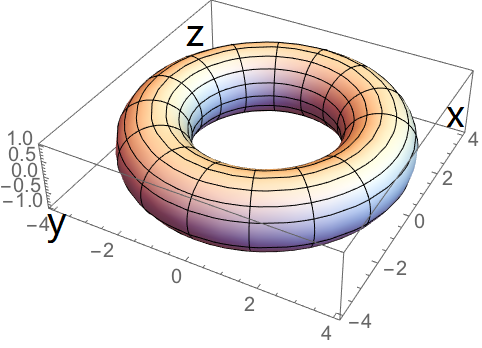
\includegraphics[scale=1]{./Pic/Torus1.png}
\caption{Torus Perspective View}
\end{figure}

\noindent
\textbf{I. Defining a Torus}

There are three circles in a torus $C_1, C_2, C_3$ as shown in the graph below. $C_2$ is how a torus is defined, because the center of the tube is uniformly lying on it and by utilizing it we can reduce our equation for the torus.  Then, we have the radius of $C_2$ as $R$ and the raidus of the tube as $r$. Therefore, we know that from this graph:
\(x^2+y^2=R^2\).
\begin{figure}[h]
\centering
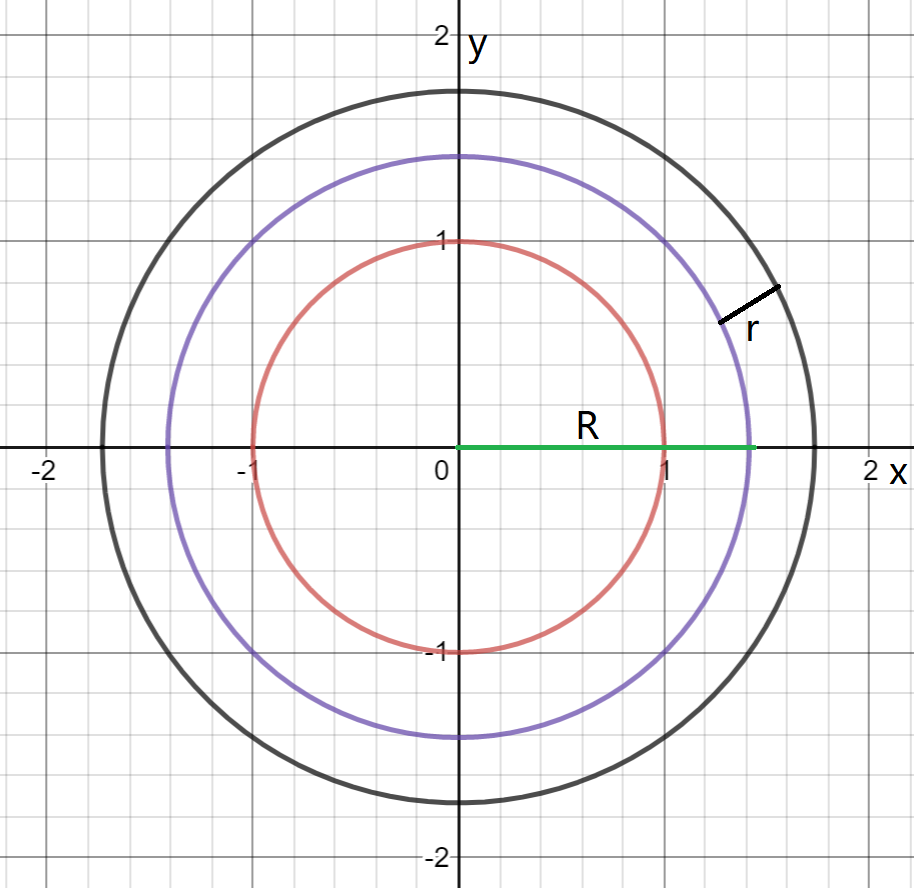
\includegraphics[scale=0.4]{./Pic/Torus2.png}
\caption{Torus Top View}
\end{figure}

Then, we just need to obtain the torus from $x,y$ and $z$. Based on observation, we can see the cross section of a torus as the following graph, and could interpret that the size of the tube should be a function like the following: $(g(x,y, R))^2+z^2=r^2$, where $g(x,y,R)$ defines where the center of a tube should lie on the middle circle.
\begin{figure}[h]
\centering
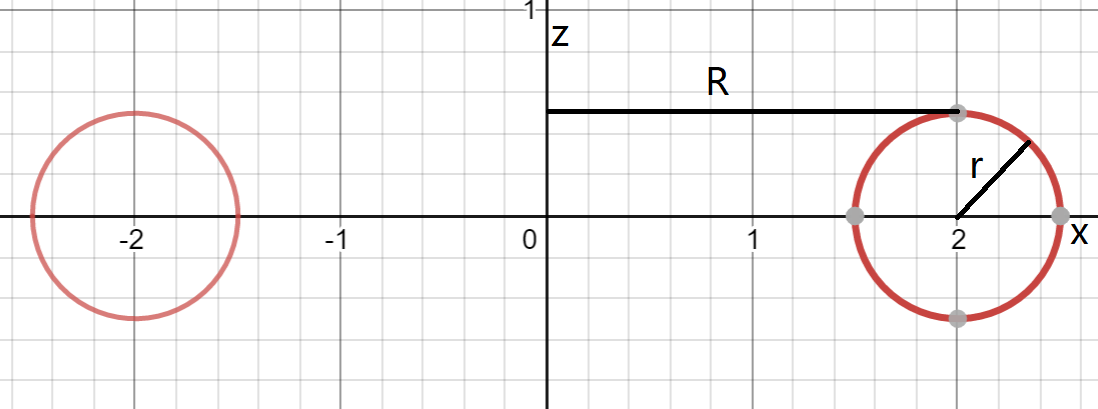
\includegraphics[scale=0.75]{./Pic/Torus3.png}
\caption{Torus Cross Section}
\end{figure}

From the previous equation we know that $x^2 +y^2 = R^2$, and we could just sample the point 
$\begin{pmatrix}
(R-r)sin\pi\\
(R-r)cos\pi\\
0
\end{pmatrix}$. This means that we should have $g(x,y,R)=\sqrt{x^2+y^2}-R$ to achieve the length of the tube. Therefore, the equation of a torus is
\begin{equation}
(\sqrt{x^2+y^2}-R)^2+z^2=r^2
\end{equation}

\noindent
\textbf{II. Finding the Intersections With a Ray}

In the ray tracer, we see each light and our camera as ray. And we define them as the following:
\begin{equation}
\overrightarrow{v} = 
\overrightarrow{o}+\overrightarrow{d}
=
\begin{pmatrix}
x_{origin}\\
y_{origin}\\
z_{origin}
\end{pmatrix} + t \cdot{
\begin{pmatrix}
x_{direction}\\
y_{direction}\\
z_{direction}
\end{pmatrix}}
\end{equation}

Thus, we have 
\begin{equation}
\begin{cases}
x=x_{origin}+t\cdot{x_{direction}}\\
y=y_{origin}+t\cdot{y_{direction}}\\
z=z_{origin}+t\cdot{z_{direction}}
\end{cases}
\end{equation}

\pagebreak
Therefore, when we define an intersection between the ray and the torus, we would have the following five situations, with 0 to 4 intersections on the torus:
\begin{figure}[h]
\centering
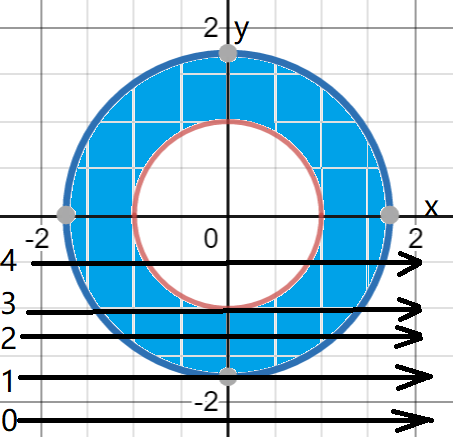
\includegraphics[scale=0.75]{./Pic/Torus4.png}
\caption{Torus Intersections on the Top View}
\end{figure}

Thus, we first rewrite (1) as the following: 
\begin{equation}
(x^2+y^2+z^2+R^2-r^2)^2=4R^2(x^2+y^2)
\end{equation}

Then, we find the intersection by replacing $x,y$ and $z$ in (4) with the equations we have in (3). Thus we have:
\begin{align*}
&((x_{origin}+t\cdot{x_{direction}})^2\\
+&(y_{origin}+t\cdot{y_{direction}})^2\\
+&(z_{origin}+t\cdot{z_{direction}})^2+R^2-r^2)^2\\
=&[(x_{direction}^2+y_{direction}^2+z_{direction}^2)t^2\\
+&2(x_{origin}x_{direction}+y_{origin}y_{direction}+z_{origin}z_{direction})t\\
+&(x_{origin}^2+y_{origin}^2+z_{origin}^2+R^2-r^2)]^2\\
=&4R^2(((x_{origin}+t\cdot{x_{direction}})^2+(y_{origin}+t\cdot{y_{direction}})^2)\\
=&4R^2((x_{direction}^2+y_{direction}^2)t^2\\
+&2(x_{origin}x_{direction}+y_{origin}y_{direction})t+(x_{origin}^2+y_{origin}^2))
\end{align*}

Since all the coefficient are constant and all of $x_{origin},y_{origin},z_{origin},x_{direction},y_{direction},z_{direction},R,r$ are constants, then we can replace all of them with certain letters for simplification. Also, we will have all these constant calculated at the beginning of our \textit{IntersectionWithRay} function. Thus, we have the following:

\[\begin{cases}
a=4R^2(x_{direction}^2+y_{direction}^2)\\
b=8R^2(x_{origin}x_{direction}+y_{origin}y_{direction})\\
c=4R^2(x_{origin}^2+y_{origin}^2)\\
d=(x_{direction}^2+y_{direction}^2+z_{direction}^2)=|\overrightarrow{d}|^2\\
e=2(x_{origin}x_{direction}+y_{origin}y_{direction}+z_{origin}z_{direction})=2(\overrightarrow{o}\cdot{\overrightarrow{d}})\\
f=(x_{origin}^2+y_{origin}^2+z_{origin}^2+R^2-r^2)=|\overrightarrow{o}|^2+R^2-r^2\\
\end{cases}\]

Then by applying all these constants back, we have: 
\begin{align*}
&a\cdot{t^2}+b\cdot{t}+c\\
=&(d\cdot{t^2}+e\cdot{t}+f)^2\\
=&d^2t^4+2det^3+(2df+e^2)t^2+2eft+f^2
\end{align*}

Therefore, we have obtained the following quartic equation for $t$:
\[d^2t^4+2dft^3+(2df+e^2-a)t^2+(2ef-b)t+f^2-c=0\]

In order to make it clearer for our definitions and calculations, we will redefine the coefficients as the following:

\[\begin{cases}
\alpha=d^2\\
\beta=2df\\
\gamma=2df+e^2-a\\
\epsilon=2ef-b\\
\omega=f^2-c\\
\end{cases}\]

Then, we rewrite the function as the following:
\[\alpha t^4+\beta t^3 + \gamma t^2 + \epsilon t + \omega = 0\]

For solving this quartic equation, we will be using a general solution, since it is not factor-able. Thus, we will need to create a few constants for solving this equation:
\[\begin{cases}
D=3\beta-8\alpha \gamma\\
E=-\beta+4\alpha\beta\gamma-8\alpha\epsilon\\
F=3\beta+16\alpha\gamma-16\alpha\beta\gamma+16\alpha\beta\epsilon-64\alpha\omega\\
A=D-3F\\
B=DF-9E\\
C=F-3DE\\
\Delta = B^2-4AC\\
\end{cases}\]
Also, we need to define another function sgn() for calculation process:

\begin{alltt}
func sgn(a float) float\{
    if a>0\{
       return float(1)
    \}
    if a == 0\{
       return float(0)
    \}
    if a<0\{
       return float(-1)    
    \}
\}
\end{alltt}
And then we would have the following cases:
\begin{alltt}
func (to Torus) IntersectWithRay(ray Ray)(count int, inters []Intersection, 
intersected bool)\{
    ...
    //All the above calculations
    //Begin cases, in pseudo code
    if D==E && D==F && D==0\{
       return 1, \(-\frac{\beta}{4\alpha}\), true
    \}
    if (D*E*F)!= 0 && A==B && B==C && A==0\{
       return 2,[\(\frac{-\beta D+9E}{4\alpha D},\frac{-\beta D-3E}{4\alpha D}\)], true
    \}
    if E==0 && E==F && D>0\{
       return 2,[\(\frac{-\beta+\sqrt{D}}{4\alpha},\frac{-\beta -\sqrt{D}}{4\alpha}\)], true
    \}
    if (A*B*C)!=0 && \(\Delta\)==0 && (A*B)>0\{
       \[\text{ans1} =\frac{-\beta+sgn(A*B*E)\sqrt{D-\frac{B}{A}}+\sqrt{\frac{2B}{A}}}{4\alpha}\]
       \[\text{ans2} =\frac{-\beta+sgn(A*B*E)\sqrt{D-\frac{B}{A}}-\sqrt{\frac{2B}{A}}}{4\alpha}\]
       \[\text{ans3} =\frac{-\beta+sgn(A*B*E)\sqrt{D-\frac{B}{A}}}{4\alpha}\]
	           return 3,[ans1,ans2,ans3],true
    \}
    if \(\Delta\) > 0 \{
	   \[z1 = AD+ \frac{3(-B+\sqrt{\Delta})}{2}\]
	   \[z2 = AD+ \frac{3(-B-\sqrt{\Delta})}{2}\]
	   \[z=D^2-D(\sqrt[3]{z1}+\sqrt[3]{z2})+(\sqrt[3]{z1}+\sqrt[3]{z2})^2-3A\]
	   \[\text{ans1}=\frac{-\beta +sgn(E)\sqrt{\frac{D+\sqrt[3]{z1}+\sqrt[3]{z2}}{3}}+\sqrt{2D-(\sqrt[3]{z1}+\sqrt[3]{z2})+2\sqrt{z}}}{4\alpha}\]
	    \[\text{ans2}=\frac{-\beta +sgn(E)\sqrt{\frac{D+\sqrt[3]{z1}+\sqrt[3]{z2}}{3}}-\sqrt{2D-(\sqrt[3]{z1}+\sqrt[3]{z2})+2\sqrt{z}}}{4\alpha}\]  
	    return 2,[ans1,ans2], true
    \}
    if \(\Delta\) < 0 && D > 0 && F > 0\{
    	    \[\theta=arccos(\frac{3B-2AD}{2A\sqrt{A}})\]
    	    \[y1=\frac{D-2\sqrt{A}cos(\frac{\theta}{3})}{3}\]
    	    \[y2=\frac{D+\sqrt{A}(cos(\frac{\theta}{3})+\sqrt{3}sin(\frac{\theta}{3}))}{3}\]
    	    \[y3=\frac{D+\sqrt{A}(cos(\frac{\theta}{3})-\sqrt{3}sin(\frac{\theta}{3}))}{3}\]
    	    if E != 0\{
           \[ans1=\frac{-\beta +sgn(E)\sqrt{y1}+\sqrt{y2}+\sqrt{y3}}{4\alpha}\]
           \[ans2=\frac{-\beta +sgn(E)\sqrt{y1}-\sqrt{y2}-\sqrt{y3}}{4\alpha}\]     
           \[ans3=\frac{-\beta -sgn(E)\sqrt{y1}+\sqrt{y2}-\sqrt{y3}}{4\alpha}\] 
           \[ans4=\frac{-\beta -sgn(E)\sqrt{y1}-\sqrt{y2}+\sqrt{y3}}{4\alpha}\] 	    
    	    \}else\{
    	        \[ans1=\frac{\beta+\sqrt{D+2\sqrt{F}}}{4a}\]
    	        \[ans2=\frac{\beta-\sqrt{D+2\sqrt{F}}}{4a}\]
    	        \[ans3=\frac{\beta+\sqrt{D-2\sqrt{F}}}{4a}\]
    	        \[ans4=\frac{\beta-\sqrt{D-2\sqrt{F}}}{4a}\]
    	    \}
    	    return 4,[ans1,ans2,ans3,ans4], true
    \}
\}
\end{alltt}
Then, we can build our intersection and computations class from these outputs and then obtain the intersections between the ray and the torus.\\

\textbf{III. Finding the Normal of the Torus}

The normal vector should be calculated from the point and the point's closest center on the xy-plane. From the graph we will see each small-circle section of the torus could be seen as a sphere that has its center sitting on the big circle on the xy-plane. 
\begin{figure}[h]
\centering
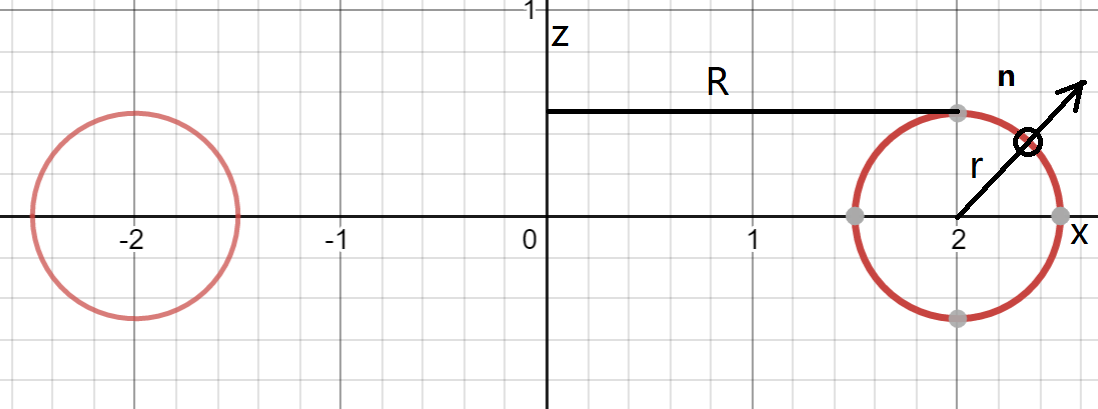
\includegraphics[scale=0.75]{./Pic/Torus5.png}
\caption{Torus Cross Section}
\end{figure}
Therefore, we will be using the following process to find the normal of a torus:

Since we are given a point $\overrightarrow{P}$ and finding the normal for the particular point. Then, we need to find center of the circle, $\overrightarrow{C}$ that is the closest to that point. Then we have  \[\overrightarrow{C}=\begin{pmatrix}
C_x\\
C_y\\
0
\end{pmatrix}\text{ and }\overrightarrow{P}=\begin{pmatrix}
P_x\\
P_y\\
P_z
\end{pmatrix}\]

These two points are all on the line with the normal $\overrightarrow{n}$ as the direction and $\overrightarrow{P}$ as the origin. Thus, $\overrightarrow{n}=\overrightarrow{P}-\overrightarrow{C}$

Then, we can project the point $\overrightarrow{P}$ on to the xy-plane. This means there should be a point $\begin{pmatrix}
P_x\\
P_y\\
0
\end{pmatrix}$ on the xy-plane that is as the same direction of $\overrightarrow{C}$ to the origin and right beneath $\overrightarrow{P}$. And we have ${C_x}^2+{C_y}^2=R^2$ which should be proportional to ${P_x}^2+{P_y}^2$. Then we can find the normal as the following:
\[\overrightarrow{n}=\begin{pmatrix}
(1-\frac{R}{\sqrt{{P_x}^2+{P_y}^2}})P_x\\
(1-\frac{R}{\sqrt{{P_x}^2+{P_y}^2}})P_y\\
P_z
\end{pmatrix}\]

And then we normalize it and convert it back to the world normal. 

\textbf{IV. Final Product}

\textbf{V. Future Development}

\end{document}
